\documentclass[12pt,a4paper]{article}
\usepackage{geometry}
\usepackage{slashbox}
\geometry{
	a4paper,
	total={170mm,257mm},
	left=20mm,
	right=20mm,
	top=20mm,
	bottom=20mm
}
\usepackage{graphicx}
\usepackage{pdfpages}
\usepackage{placeins}
\usepackage{float}

\usepackage{polski}
\usepackage[utf8]{inputenc}

\begin{document}
	
	\begin{titlepage}
		\newgeometry{top=5.5cm, bottom=3cm}
		
		\centering
		{\huge\bfseries Logika układów cyfrowych lab.\par}
		
		\vspace{0.5cm}
		Prowadzący: Mgr inż. Antoni Sterna (E02-38m, wtorek 17:05) \\
	
		\vspace{1.1cm}
		{\Large sprawozdanie 4 - 2017.11.07\par}
		\vfill
		
		{\large\bfseries Jakub Dorda 235013\par}
		{\large\bfseries Marcin Kotas 235098\par}
		
		\vspace{1cm}
		\today \\ \LaTeX
		
		\restoregeometry
	\end{titlepage}

	
	\section{Wprowadzenie/cel ćwiczeń}
	
	
		
	\section{Licznik synchroniczny 3 bitowy rewersyjny}
		
		\subsection{Tabela prawdy i tablice Karnaugh:}
			\begin{table}[H]
				\caption{Tabela Prawdy}
				\vspace{0.2cm}
				\centering
				\begin{tabular}{cccc|ccc|cc|cc|cc}
					A	&\(Q_2\)&\(Q_1\)&\(Q_0\)&\(Q_2^+\)&\(Q_1^+\)&\(Q_0^+\)&\(J_2\)&\(K_2\)&\(J_1\)&\(K_1\)&\(J_0\)&\(K_0\)\\\hline
					0	&	0	&	0	&	0	&	0	&	0	&	1	&	0	&	-	&	0	&	-	&	1	&	-	\\
					0	&	0	&	0	&	1	&	0	&	1	&	0	&	0	&	-	&	1	&	-	&	-	&	1	\\
					0	&	0	&	1	&	0	&	0	&	1	&	1	&	0	&	-	&	-	&	0	&	1	&	-	\\
					0	&	0	&	1	&	1	&	1	&	0	&	0	&	1	&	-	&	-	&	1	&	-	&	1	\\\hline
					0	&	1	&	0	&	0	&	1	&	0	&	1	&	-	&	0	&	0	&	-	&	1	&	-	\\
					0	&	1	&	0	&	1	&	1	&	1	&	0	&	-	&	0	&	1	&	-	&	-	&	1	\\
					0	&	1	&	1	&	0	&	1	&	1	&	1	&	-	&	0	&	-	&	0	&	1	&	-	\\
					0	&	1	&	1	&	1	&	0	&	0	&	0	&	-	&	1	&	-	&	1	&	-	&	1	\\\hline
					1	&	0	&	0	&	0	&	1	&	1	&	1	&	1	&	-	&	1	&	-	&	1	&	-	\\
					1	&	0	&	0	&	1	&	0	&	0	&	0	&	0	&	-	&	0	&	-	&	-	&	1	\\
					1	&	0	&	1	&	0	&	0	&	0	&	1	&	0	&	-	&	-	&	1	&	1	&	-	\\
					1	&	0	&	1	&	1	&	0	&	1	&	0	&	0	&	-	&	-	&	0	&	-	&	1	\\\hline
					1	&	1	&	0	&	0	&	0	&	1	&	1	&	-	&	1	&	1	&	-	&	1	&	-	\\
					1	&	1	&	0	&	1	&	1	&	0	&	0	&	-	&	0	&	0	&	-	&	-	&	1	\\
					1	&	1	&	1	&	0	&	1	&	0	&	1	&	-	&	0	&	-	&	1	&	1	&	-	\\
					1	&	1	&	1	&	1	&	1	&	1	&	0	&	-	&	0	&	-	&	0	&	-	&	1	\\
					\end{tabular}
			\end{table}
			\begin{table}[H]
				\begin{minipage}{.5\textwidth}
					\caption{Tablica Karnaugh dla $J_2$}
					\vspace{0.2cm}
					\centering
					\begin{tabular}{c|c|c|c|c}
						\backslashbox{$AQ_2$}{$Q_1Q_0$}&00&01&11&10\\\hline
						00	&	0	&	0	&	1	&	0	\\\hline
						01	&	-	&	-	&	-	&	-	\\\hline
						11	&	-	&	-	&	-	&	-	\\\hline
						10	&	1	&	0	&	0	&	0	
					\end{tabular}
				
					\caption{Tablica Karnaugh dla $J_1$}
					\vspace{0.2cm}
					\centering
					\begin{tabular}{c|c|c|c|c}
						\backslashbox{$AQ_2$}{$Q_1Q_0$}&00&01&11&10\\\hline
						00	&	0	&	1	&	-	&	-	\\\hline
						01	&	0	&	1	&	-	&	-	\\\hline
						11	&	1	&	0	&	-	&	-	\\\hline
						10	&	1	&	0	&	-	&	-	
					\end{tabular}
				
					\caption{Tablica Karnaugh dla $J_0$}
					\vspace{0.2cm}
					\centering
					\begin{tabular}{c|c|c|c|c}
						\backslashbox{$AQ_2$}{$Q_1Q_0$}&00&01&11&10\\\hline
						00	&	-	&	-	&	-	&	-	\\\hline
						01	&	0	&	0	&	1	&	0	\\\hline
						11	&	1	&	0	&	0	&	0	\\\hline
						10	&	-	&	-	&	-	&	-	
					\end{tabular}
				\end{minipage}%
				\begin{minipage}{.5\textwidth}
					\caption{Tablica Karnaugh dla $K_2$}
					\vspace{0.2cm}
					\centering
					\begin{tabular}{c|c|c|c|c}
						\backslashbox{$AQ_2$}{$Q_1Q_0$}&00&01&11&10\\\hline
						00	&	0	&	0	&	1	&	0	\\\hline
						01	&	-	&	-	&	-	&	-	\\\hline
						11	&	-	&	-	&	-	&	-	\\\hline
						10	&	1	&	0	&	0	&	0	
					\end{tabular}
					
					\caption{Tablica Karnaugh dla $K_1$}
					\vspace{0.2cm}
					\centering
					\begin{tabular}{c|c|c|c|c}
						\backslashbox{$AQ_2$}{$Q_1Q_0$}&00&01&11&10\\\hline
						00	&	-	&	-	&	1	&	0	\\\hline
						01	&	-	&	-	&	1	&	0	\\\hline
						11	&	-	&	-	&	0	&	0	\\\hline
						10	&	-	&	-	&	0	&	1	
					\end{tabular}
					
					\caption{Tablica Karnaugh dla $K_0$}
					\vspace{0.2cm}
					\centering
					\begin{tabular}{c|c|c|c|c}
						\backslashbox{$AQ_2$}{$Q_1Q_0$}&00&01&11&10\\\hline
						00	&	-	&	1	&	1	&	-	\\\hline
						01	&	-	&	1	&	1	&	-	\\\hline
						11	&	-	&	1	&	1	&	-	\\\hline
						10	&	-	&	1	&	1	&	-	
						
					\end{tabular}
				\end{minipage}
			\end{table}
			
			
		\subsection{Minimalizacje:}
			
			\begin{displaymath}
			J_2 = K_2 = A\bar{Q_1}\bar{Q_0} + \bar{A}Q_1Q_0 = \overline{\overline{A\bar{Q_1}\bar{Q_0}} \cdot \overline{\bar{A}Q_1Q_0}}
			\end{displaymath}
			\begin{displaymath}
			J_1 = K_1 = \bar{A}Q_0 + A\bar{Q_0}= \overline{\overline{\bar{A}Q_0} \cdot \overline{A\bar{Q_0}}}
			\end{displaymath}
			\begin{displaymath}
			J_0 = K_0 = 1
			\end{displaymath}
		
		
		\subsection{Użyte wzory:}
		
		\begin{equation}
		\overline{a\cdot b}=\bar{a}+\bar{b}
		\end{equation}
		\begin{equation}
		\overline{a+b}=\bar{a}\cdot\bar{b}
		\end{equation}

		\subsection{Schemat układu:}
		
			\vspace{1.5cm}
			\begin{center}
				\makebox[\textwidth]{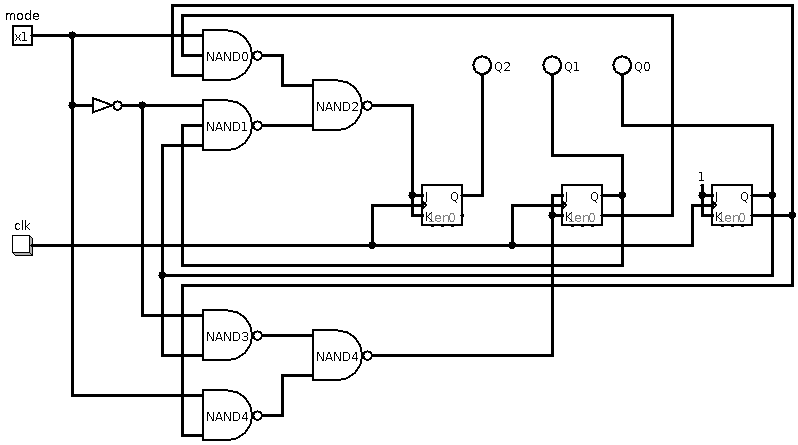
\includegraphics[width=\paperwidth - 30mm]{schem/circuit.png}}
				Schemat 1: 
			\end{center}
	
	\section{Licznik asynchroniczny modulo 4/11}
		
		\subsection{Tabela prawdy i tablice Karnaugh:}
			\begin{table}[H]
				\begin{minipage}{.5\textwidth}
					\caption{Tabela Prawdy cz.1}
					\vspace{0.2cm}
					\centering
					\begin{tabular}{ccccc|c}
						M	&\(Q_3\)&\(Q_2\)&\(Q_1\)&\(Q_0\)&	R	\\\hline
						0	&	0	&	0	&	0	&	0	&	1	\\
						0	&	0	&	0	&	0	&	1	&	1	\\
						0	&	0	&	0	&	1	&	0	&	1	\\
						0	&	0	&	0	&	1	&	1	&	1	\\\hline
						0	&	0	&	1	&	0	&	0	&	0	\\
						0	&	0	&	1	&	0	&	1	&	0	\\
						0	&	0	&	1	&	1	&	0	&	0	\\
						0	&	0	&	1	&	1	&	1	&	0	\\\hline
						0	&	1	&	0	&	0	&	0	&	0	\\
						0	&	1	&	0	&	0	&	1	&	0	\\
						0	&	1	&	0	&	1	&	0	&	0	\\
						0	&	1	&	0	&	1	&	1	&	0	\\\hline
						0	&	1	&	1	&	0	&	0	&	-	\\
						0	&	1	&	1	&	0	&	1	&	-	\\
						0	&	1	&	1	&	1	&	0	&	-	\\
						0	&	1	&	1	&	1	&	1	&	-	\\
					\end{tabular}
				\end{minipage}%
				\begin{minipage}{.5\textwidth}
					\caption{Tabela Prawdy cz.2}
					\vspace{0.2cm}
					\centering
					\begin{tabular}{ccccc|c}
						M	&\(Q_3\)&\(Q_2\)&\(Q_1\)&\(Q_0\)&	R	\\\hline
						1	&	0	&	0	&	0	&	0	&	1	\\
						1	&	0	&	0	&	0	&	1	&	1	\\
						1	&	0	&	0	&	1	&	0	&	1	\\
						1	&	0	&	0	&	1	&	1	&	1	\\\hline
						1	&	0	&	1	&	0	&	0	&	1	\\
						1	&	0	&	1	&	0	&	1	&	1	\\
						1	&	0	&	1	&	1	&	0	&	1	\\
						1	&	0	&	1	&	1	&	1	&	1	\\\hline
						1	&	1	&	0	&	0	&	0	&	1	\\
						1	&	1	&	0	&	0	&	1	&	1	\\
						1	&	1	&	0	&	1	&	0	&	1	\\
						1	&	1	&	0	&	1	&	1	&	0	\\\hline
						1	&	1	&	1	&	0	&	0	&	-	\\
						1	&	1	&	1	&	0	&	1	&	-	\\
						1	&	1	&	1	&	1	&	0	&	-	\\
						1	&	1	&	1	&	1	&	1	&	-	\\
					\end{tabular}
				\end{minipage}
			
				\caption{Tablica Karnaugh dla $R$}
				\vspace{0.2cm}
				\centering
				\begin{tabular}{c|c|c|c|c|c|c|c|c}
					\backslashbox{$Q_2$}{$Q_1Q_0$}&000&001&011&010&110&111&101&100\\\hline
					00	&	1	&	0	&	-	&	0	&	1	&	-	&	1	&	1	\\\hline
					01	&	1	&	0	&	-	&	0	&	1	&	-	&	1	&	1	\\\hline
					11	&	1	&	0	&	-	&	0	&	0	&	-	&	1	&	1	\\\hline
					10	&	1	&	0	&	-	&	0	&	1	&	-	&	1	&	1	
					
				\end{tabular} 
			\end{table}
		\subsection{Minimalizacje:}
			
			\begin{displaymath}
			R = \bar{Q_3}\bar{Q_2} + M\bar{Q_3} + M\bar{Q_1} + MQ_1\bar{Q_0} = \overline{\overline{\bar{Q_3}\bar{Q_2}} \cdot \overline{M\bar{Q_3}} \cdot \overline{M\bar{Q_1}} \cdot \overline{MQ_1\bar{Q_0}}}
			\end{displaymath}
			
		\subsection{Użyte wzory:}
		
			\begin{equation}
			\overline{a+b}=\bar{a}\cdot\bar{b}
			\end{equation}
			
		\subsection{Schemat układu:}
		
			\vspace{0.5cm}
			\begin{center}
				\makebox[\textwidth]{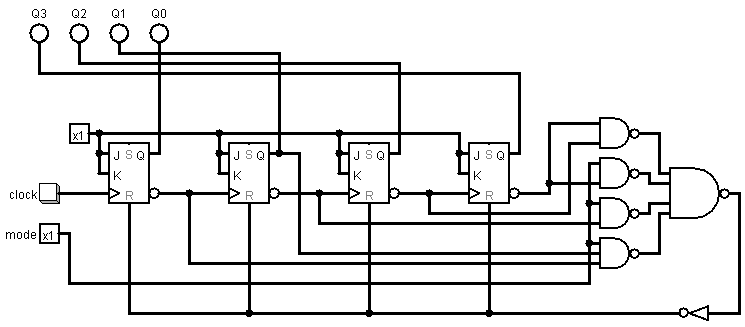
\includegraphics[width=\paperwidth - 20mm]{schem/circuit2v3(final).png}}
				Schemat 2: 
			\end{center}

	\section{Wnioski/podsumowanie}
	
	
\end{document}